\RequirePackage[orthodox]{nag}
\documentclass[11pt]{article}

%% Define the include path
\makeatletter
\providecommand*{\input@path}{}
\g@addto@macro\input@path{{include/}{../../include/}}
\makeatother

\usepackage{../../include/akazachk}

\title{Computer Security - 80156}
\author{Andres Espinosa}
\begin{document}
\pgfplotsset{compat=1.18}
\maketitle

\tableofcontents

\section{Introduction}
\subsection{Motivation of Computer Security}
As computers and the relationships between them have evolved, computers have grown to be an interconnected network of devices, machines, data, transactions, and other systems.
By limiting the access that different computers and different users have to these systems we can enforce a level of protection across this network.
We are therefore motivated to improve these security processes and protocols to ensure we can protect computer and information systems across the world with little barrier of entry.

\subsection{What is Information Security?}
\textbf{Computer Security} deals with the prevention and detection of \textit{unauthorized} actions by user of a computer system.
The term \textit{authorization} allows us to crucially define different actors and agents that we \textit{authorize} to use our system.
A simple example, we create our phone password and at times we share it with one or two other trusted users, these users then become \textit{authorized} users of the system.
This in effect becomes our \textit{security policy}, a set of rules and information that dictate who (or what) may perform which actions in a computer system.

\textbf{Information Security} is even more general, it deals with \textit{information} independent of computer systems.
Information can be any type of numbers, facts, or words displayed or communicated by a computer system.
Typically, information is important strings, data, or summaries that should be protected. 

To protect our right of proctection of self, we have developed these fields of information and computer security accordingly.

Some key concepts of information security include the following:

\begin{itemize}
    \item \textbf{Security} concerns the protection of \textbf{assets} from \textbf{threats}
    \item \textbf{Threats} are the potential of abuse of \textbf{assets}
    \item \textbf{Owners} value their \textbf{assets} and want to protect them
    \item \textbf{Threat agents} also value \textbf{assets}, and serve as adversarial entities that seek to abuse an owner's \textbf{assets}
    \item Although many \textbf{threat agents} may exist, those that the \textbf{owner} is able to determine as significant are \textbf{risks}
    \item \textbf{Risks} can result in numerous \textbf{vulnerabilities} to a system, and \textbf{countermeasures} can be employed to reduce them and ideally minimize them (keeping in mind a tradeoff with feasibility and expense)
\end{itemize}

\subsection{Security Properties}
There are a few properties that define how secure an information or computer system is.

\begin{enumerate}
    \item \textbf{confidentiality} information is not learned by unauthorized principals
    \item \textbf{integrity} data has not been (maliciously) altered
    \item \textbf{authentication} principals or data origin can be identified accurately
    \item \textbf{availability} data/services can be accessed when desired
    \item \textbf{accountability} actions can be trace to responsible principals
\end{enumerate}

Systems typically require a great deal of protection on these properties holistically throughout the system.
We can't narrow in or tunnel vision to a specific property (confidentiality, integrity, etc) on a specific part of the system (hardware, software, etc) as security is a whole system issue.
In order to protect these properties, we implement protection countermeasures in the following section.

\subsubsection{Countermeasures}
\textbf{Prevention}. 
The goal of the prevention countermeasure is to intelligently design the system and employ appropriate security technologies to prevent security breaches from occurring in the first place.
For example, a firewall set up to prevent external access to corporate intranets which immediately checks and forces appropriate credentials login before a user accesses the intranet.

\textbf{Detection}.
In the event of a security breach, we try to ensure that it will be detected.
Logging and MACs (file hashes to detect alteration) are primary methods of detection to identify when a security breach has occurred.
There exist intrusion detection systems which actively watch for intruders which are more common detection methods in practice.

\textbf{Response}.
In the event of a secuirty breach, we must respond or recover the assets.
Responses range from restoring backups through to informing appropriate concerned parties or law-enforcement agencies.

\subsubsection{Protecting Properties}
\textbf{Confidentiality}, in general, is concerned with an unauthorized learning of information.
Clearly, this can mean many different things in different systems and agents.
One such example can be someone using unauthorized access to read data they otherwise would not be able to do.
Confidentiality presumes a notion of an authorized party, or more generally, a \textit{security policy} with rules that dictate who or what can access our data (and appropriate when/where conditions for that access).
Confidentiality is also closely related to the ideas of privacy and secrecy, the former generally meaning confidentiality for individuals and the latter meaning confidentiality for organizations or groups of individuals.
For example, a medical record obtained without your consent is a confidentiality breach that infringes on your privacy.
\\ \\
\textbf{Integrity}, in the context of computer security, means the ability of the system's information to be maliciously altered by someone who is not authorized to do so.
Integrity can be thought of as the \textit{write} counterpart to confidentiality's \textit{read}.
An example could be a payment that was maliciously altered and increased from 100 euro to 10.000 euro.
\\ \\
\textbf{Authentication} is verification of the identity of a person or system.
In the event that a system wishes to grant access to certain individuals while simultaneously restricting access to others, authentication is a crucial piece with an access control system.
Different methods of authentication can be: entrycards, RFID, passwords, fingerprint, passkeys, etc.
Depending on the system, different checking methods can be used: either implicity or explicitly checked.
We can have a process running in the background that ensures that a user is logged in at each new HTTP request, or we can force the user to login each time they enter a site.
Different authentication methods can be compounded on each other as well to implicitly and explicitly check in multiple ways to increase the level of security.
For example, we could run an explicit username and password check to have a user login, then implicitly verify their status as a "subscribed" member.
\\ \\
\textbf{Availability} ensures that a service can be accessed in a reliable and timely way.
Different systems require different levels of availability depending on their purposes.
A threat to availability covers many different kinds environmental events (fire, power outage, etc) and also incidental malicious attacks (virus, DoS attacks)
By ensuring availability we attempt to prevent \textit{denial of service} (DoS) attacks, as much as possible.
An example violation of the availability property is a deadly distributed DoS attack against an on-line service to render it impossible to be used.
\\ \\
\textbf{Accountability} means that actions are recorded and can be traced to the party responsible.
When prevention methods and access controls fail (or are too expensive), we can fall back to detection: keeping a \textit{secure audit trail} is important so that actions affecting security can be traced back to the responsible party.
If the level of accountability is strong enough, it is \textit{non-repudiation}, when a party does not have a plausible deniability to that action.
Logs must be safe and should not be able to be tampered with so are often sent to a location that is isolated and append-only.

\subsection{Implementing a Security Solution}
\begin{itemize}
    \item A \textbf{security analysis} surveys the threats which pose risks to assets, and then proposes policy and solutions at an appropriate cost.
    \item A \textbf{threat model} documents the possible threats to a system, imagining all the vulnerabilities which might be exploited.
    \item A \textbf{risk assessment} studies the likelihood of each threat in the system environment and assigns a cost value, to find the risks.
    \item A \textbf{security policy} addresses the threats, and describes a coherent set of \textit{countermeasures}.
    \item This allows a \textbf{security solution} to be designed, deploying appropriate technologies at an appropriate cost.
          Partly this is a budgeting exercise; but it's also important to spend effort in the right place.
\end{itemize}

\subsection{Cyber-risk}
Risk is the way that we determine how harmful and likely a threat is.
With a given event $e$, the risk of that event is determined by its likelihood and impact.
\begin{equation}
    \text{Risk}_e = \text{Likelihood}_e \times \text{Impact}_e
\end{equation}

A system/organization may have numerous potential events $e$ that pose security risks.
We can evaluate and sum all individual risks to identify the total risk exposure to a system.
The treatment and mitigation of risks is naturally a cost/time tradeoff with security.
It is therefore necessary to evaluate risks sufficiently to identify which countermeasures are worth the cost of implementation and deployment.

\subsubsection{Cyber-risk Management}
NIST has a framework for managing cyber-risk that divides into 5 core function.
\begin{itemize}
    \item Recover
    \item Identify: Develop an organizational understanding to manage cybersecurity risk to systems.
    \item Protect: Develop and implement the appropriate safeguards to ensure delivery of service.
    \item Detect: 
    \item Respond
\end{itemize}

\textbf{Identify}: Develop an organizational understanding to manage cybersecurity risk to systems.
Identifying a risk is important to manage cyber-risk because we can establish policies that build roles and responsibilities for users.
Things like dual factor authentication is a way to increase the governance in our identification process.

\textbf{Protect}: Develop and implement the appropriate safeguards to ensure delivery of service.
There are many systems put in place to protect a system.
\begin{itemize}
    \item Firewall: A firewall is a line of defense that aims to guard the junctions of a piece of digital infrastructure. 
          By protecting these crucial areas and ensuring that data sent follows the security policy, we can decrease the risks associated with not following our security policy.
    \item Anti-virus: An anti-virus is a program that automatically scans files in a network for any sources of potential harm.
    \item Intrusion Prevention Systems: An IPS polices a network and monitors traffic to actively block any malicious activity.
    \item Identity and Access Management Systems: An IAMS is a program set up to centrally contain users and their permissions. 
          We then validate and ensure that all users in a system are limited to their permissions and are present in the system.
\end{itemize}

\textbf{Detect}: Develop and implement the appropriate activities to identify the occurence of a cybersecurity event.
Intrusion detection systems exist that do not actively block actions but attempt to detect and flag any potentially harmful intrusions.

\textbf{Respond}: Develop and implement the appropriate activities to take action regarding a detected cybersecurity event.
Do we have a system in place to quickly respond to a cybersecurity incident?

\textbf{Recover}: Develop and implement the appropraite activities to maintain plans for resilience and to restore any capabilities or services that were impaire due to a cybersecurity event.
Backups are an important way for us to quickly recover and revert back to a version prior to the cybersecurity incident.

\section{Cryptography}

\subsection{Introduction}

Preserving information and its security as we pass it along is one of the oldest cybersecurity problems.
As we open channels between communication partners, we want to make sure that we keep the information intact and untampered with.
How do we turn \textbf{untrustworthy channels} into \textbf{trustworthy} ones?
Cryptography is the enabling technology that allows us to preserve the confidentiality, integrity, and authentication as we pass information.

Cryptology is the study of secret writing, steganography is the science of hiding messages in other messages, and cryptography is the science of secret writing.

\begin{figure}[htbp]
  \centerline{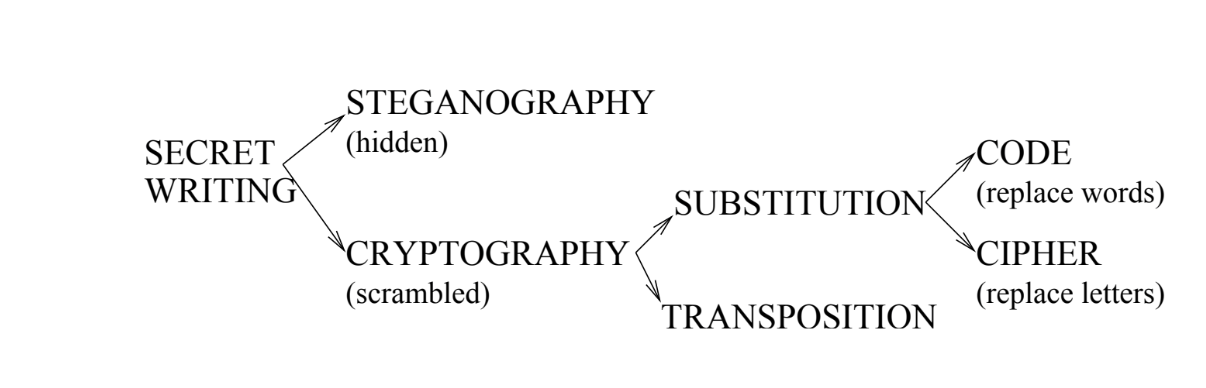
\includegraphics[width=0.75\textwidth]{../../images/cryptography_diagram.png}}
  \caption{A diagram of the workings of cryptography}
  \label{fig:cryptography_diagram}
\end{figure}

\begin{figure}[htbp]
  \centerline{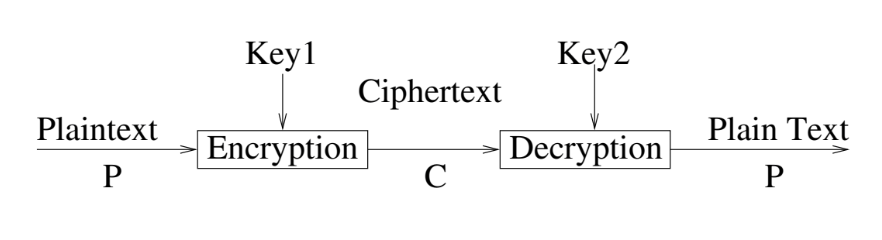
\includegraphics[width=0.75\textwidth]{../../images/general_cryptography_schema.png}}
  \caption{The general cryptography schema}
  \label{fig:general_cryptography_schema}
\end{figure}

\begin{itemize}
    \item \textbf{Security depends on secrecy of the key, not of the algorithm}
    \item An algorithm is symmetric if key1 is equal to key2 or are easily derived from each other.
    \item An algorithm can be asymmetric or public key if they are different keys that cannot be derived frome ach other or there is one key that is public and can be published without compromising the private key.
\end{itemize}

Communicating the key is crucial to occur over a secure channel and is one of the fundamental problems of cybersecurity.

There exist two classifications of security: unconditional and conditional.
Unconditional security means that a system is secure even if an adversary has infinite computing power.
This occurs when the ciphertext provides insufficient information to uniquely determine the corresponding plaintext.
Conditional security entails an adversary having a theoretic ability to calculate the plaintext from the ciphertext, however this would require more power than any adversary would realistically have.

A brute-force attack is a method of attempting to decrypt which would involve trying every key.

There are a few kinds of attacks.
A \textbf{ciphertext only} attack starts with the cipher text given and attempts to deduce the original plaintext message.
Given $C_1 = E_k (M_1), \dots, C_n E_k (M_n)$ deduce $M_1, \dots, M_n$.
Another type of attack is a \textbf{known plaintext} attack, where the attacker knows the plaintext message and the cipher text.
Their goal is to get the key or to compute the algorithm to be able to decrypt future messages even when they do not have the future plaintext.
Given $M_1, C_1 = E_k (M_1), \dots, M_n, C_n E_k (M_n)$ deduce $M_{n+1} from C_{n+1} = E_k (M_{n+1})$.

\subsection{Mathematical formulation}
\begin{itemize}
    \item $A$, is the alphabet, the finite set of characters.
    \item $M \subseteq A^*$ is the message space. $\textbf{M} \in M $ is a plaintext message.
    \item $C$ is the ciphertext space, whose alphabet could differ from $M$.
    \item $K$ denotes the key space of keys.
    \item Each $e \in K$ determines a bijective function from $M \to C$, denoted by $E_e$. $E_e$ is the encryption function.
    \item Similarly, for each $d \in K$, $D_d$ (the decryption function) denotes a bijection from $C \to M$.
\end{itemize}

An encryption scheme or cipher consists of an encrypting set $\{ E_e | e \in K \}$ and a corresponding decrypting set $ \{ D_d | d \in K \}$ with the property that for each $e \in K$ there is a unique $d \in K$ such that $D_d = E_e^{-1}$
\begin{equation}
    D_d(E_e(m)) = m, \quad \forall m \in M
\end{equation}

The keys $(e,d)$ form a key pair.

To construct an encryption scheme requires fixing a message space $M$, a ciphertext space $C$, and a key space $K$, as well as encryption transformations $\{ E_e | e \in K \}$ and corresponding decryption transformations $\{ D_d | d \in K  \}$

\subsection{Symmetric-key encryption}
Consider a cipher $\{ E_e | e \in K \}, \{ D_d | d \in K  \}$.
The cipher is symmetric-key if for each associated pair $(e,d)$ it is computationally "easy" to determine $d$ knowling only $e$ and to determine $e$ from $d$.
In practice, it is symmetric-key if $e=d$.
In symmetric-key, the sender and recipient share a common key for both encryption and decryption.
Transmitting the symmetric-key is frequently a major problem with this cipher type.

\subsubsection{Block vs Stream vs Codes}
There are a few types of cipher / encryption scheme types that define how the cipher breaks up messages of different lengths.
\begin{itemize}
    \item A \textbf{block cipher} works by breaking up a long plaintext message into different blocks of a fixed length $t$ and it encrypts each block one at a time.
    \item A \textbf{stream cipher} is a block cipher where the block-length is 1. It therefore breaks up by each character.
    \item A \textbf{code} does not care about the specific length of a word and encrypts word-by-word.
\end{itemize}

\subsection{Substitution Ciphers}

Substitution ciphers work by directly substituting characters for other characters in an attempt to conceal the original message.
\begin{itemize}
    \item Caesar Cipher: Rotate each character by three alphabet characters to the right: "HELLO WORLD" $\longrightarrow$ "KHOOR ZRUOG"
    \item ROT13: Same process as the Caesar Cipher but by 13 places
    \item Alphanumeric: Substituting numbers for letters: "2-25-5" $\longrightarrow$ "BYE".
\end{itemize}

A mono-alphabetic substiution cipher is the generalized version of a caesar cipher where each substitution is set in the key arbitrarily.
An affine cipher is  mono-alphabetic substitution cipher that follows the formula 
\begin{equation}
    e(m) = (am + b) \% |A|
\end{equation}
where \% is the modulus operator.

A problem frequently occurs with substitution ciphers due to the fact that any written language has a probability distribution on its characters.
With a long enough ciphertext that has been encrypted through mono-alphabetic substitution, it is generally possible to count relative letter frequencies and use trial and error to decipher the key.


Homophonic substitution ciphers exist which replace each alphabet character $a$ with a randomly chosen string from $H(a)$.
Where $H(a)$ is a set of strings of $t$ symbols.



\end{document}